\documentclass[]{final_report}
\usepackage{graphicx}
\usepackage{hyperref}


%%%%%%%%%%%%%%%%%%%%%%
%%% Input project details
\def\studentname{Luke Sell}
\def\reportyear{2019}
\def\projecttitle{Playing Games and Solving Puzzles Using AI}
\def\supervisorname{Iddo Tzameret}
\def\degree{BSc (Hons) in Computer Science}
\def\fullOrHalfUnit{Full Unit} % indicate if you are doing the project as a Full Unit or Half Unit
\def\finalOrInterim{User Interface Design for a solver} % indicate if this document is your Final Report or Interim Report

\begin{document}

\maketitle

%%%%%%%%%%%%%%%%%%%%%%
%%% Declaration

\chapter*{Declaration}

This report has been prepared on the basis of my own work. Where other published and unpublished source materials have been used, these have been acknowledged.

\vskip3em

Word Count: N/A

\vskip3em

Student Name: \studentname

\vskip3em

Date of Submission: 05/10/2019

\vskip3em

Signature: l.sell

\newpage

%%%%%%%%%%%%%%%%%%%%%%
%%% Table of Contents
\tableofcontents\pdfbookmark[0]{Table of Contents}{toc}\newpage

The User Interface for the application needs to be easy to understand and usable by the user, it should also help them and make clear what the grid is representing so they can solve the Sudoku.

The buttons that the user can use are to the side of the grid with the main grid in the centre, the grid itself has lines drawn to separate the squares with dotted lines to represents the separation between squares within a box. Squares that are not yet filled in are shown as empty rather than their object representation of zero to make it easier for the user to see which squares have not yet been solved. The initial starting numbers given are locked and displayed with a grey overlay so that the user knows which squares these are and that they cannot modify them. The user can also select squares which highlights them in green. When the grid is solved all squares are locked so that the user cannot accidentally modify squares and invalidate the completed grid.

To improve the UI and User Experience when using the application, I will also allow the user to use the arrow keys to move between squares and select them, and will also allow the user to undo a modification to set a square back to a previous number easily. To make it more clear which row, column or box a square is in, I will also highlight those other squares in another colour. I will also allow the user to right click a square to select it for making notes on possible numbers, these can then be modified as the user attempts to solve the Sudoku as the constraints propagate, these would be displayed above the centre of the square in smaller font.

\newpage

\begin{figure}[h]
	\centering
	\fboxsep 2mm
	\framebox{
		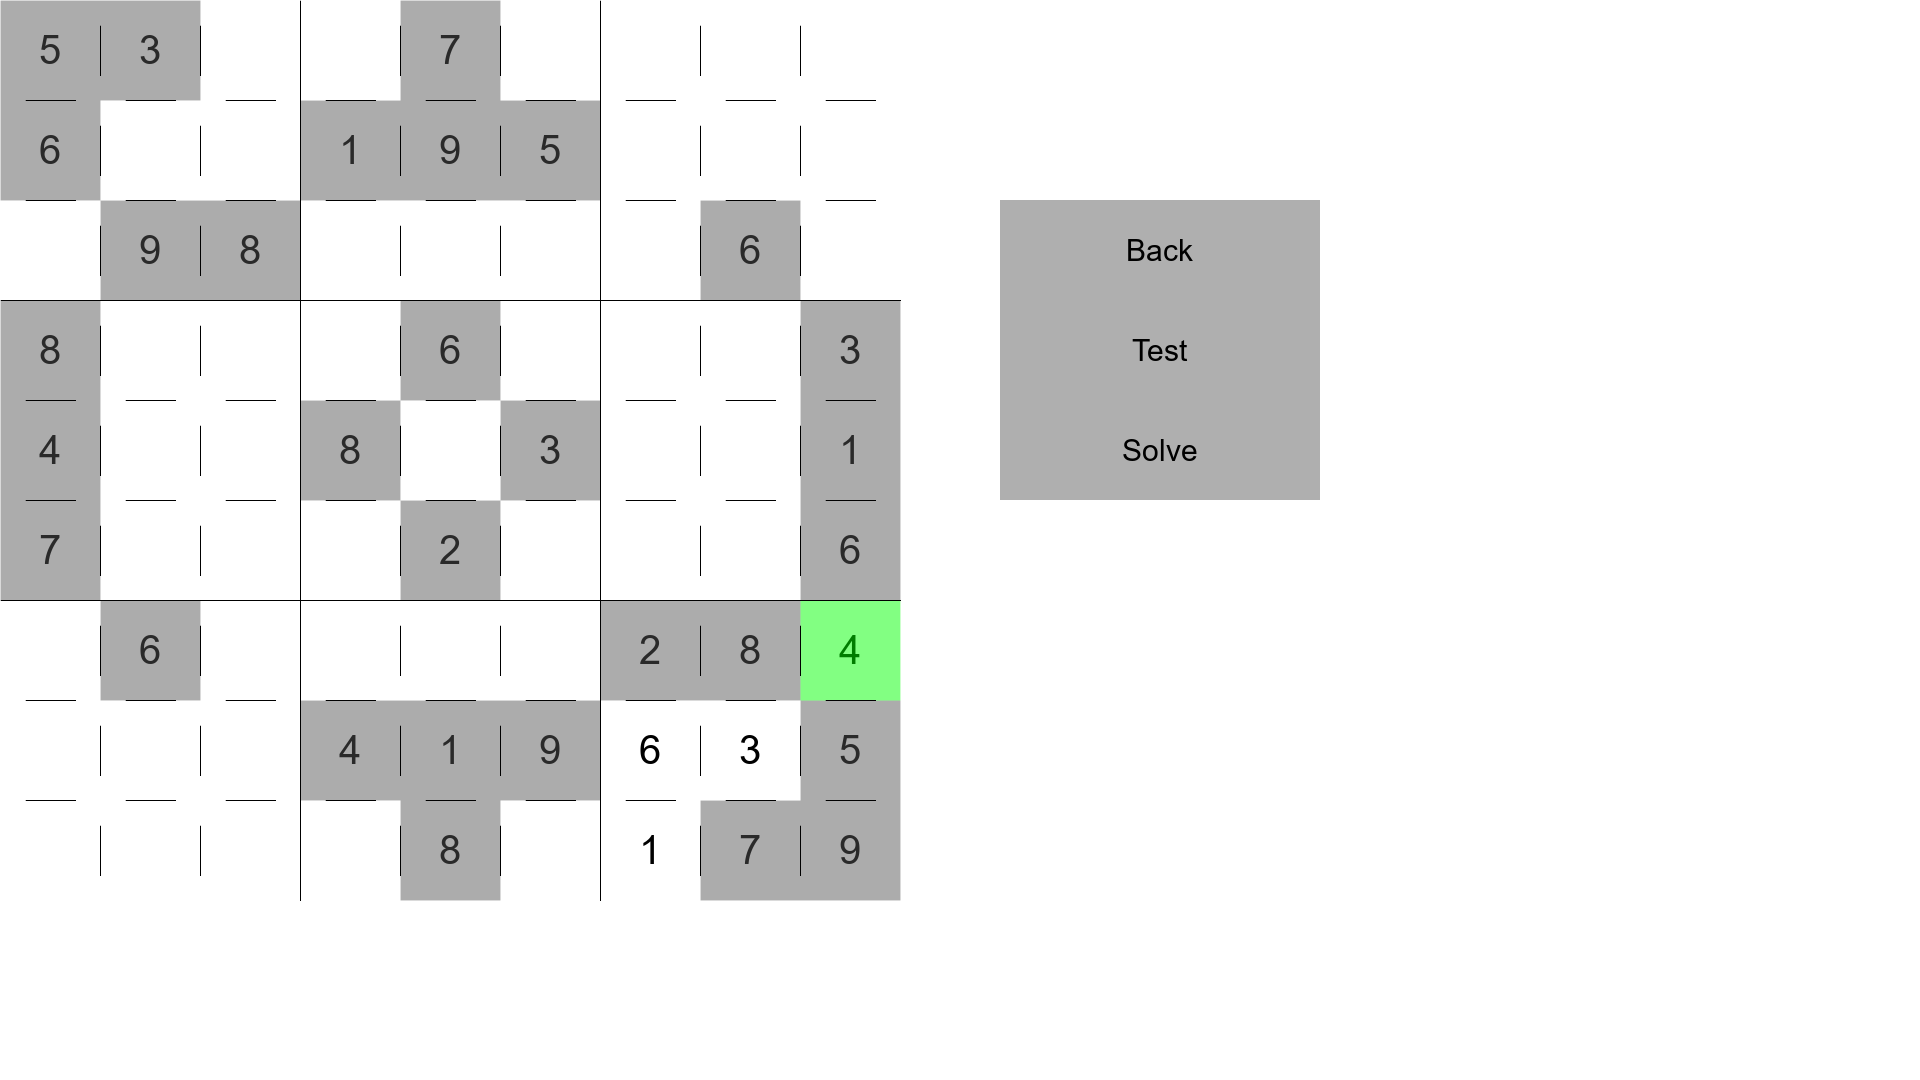
\includegraphics[width=14cm]{user} 
	}
	\caption{\label{fig:user} User Input.}
\end{figure}

\begin{figure}[h]
	\centering
	\fboxsep 2mm
	\framebox{
		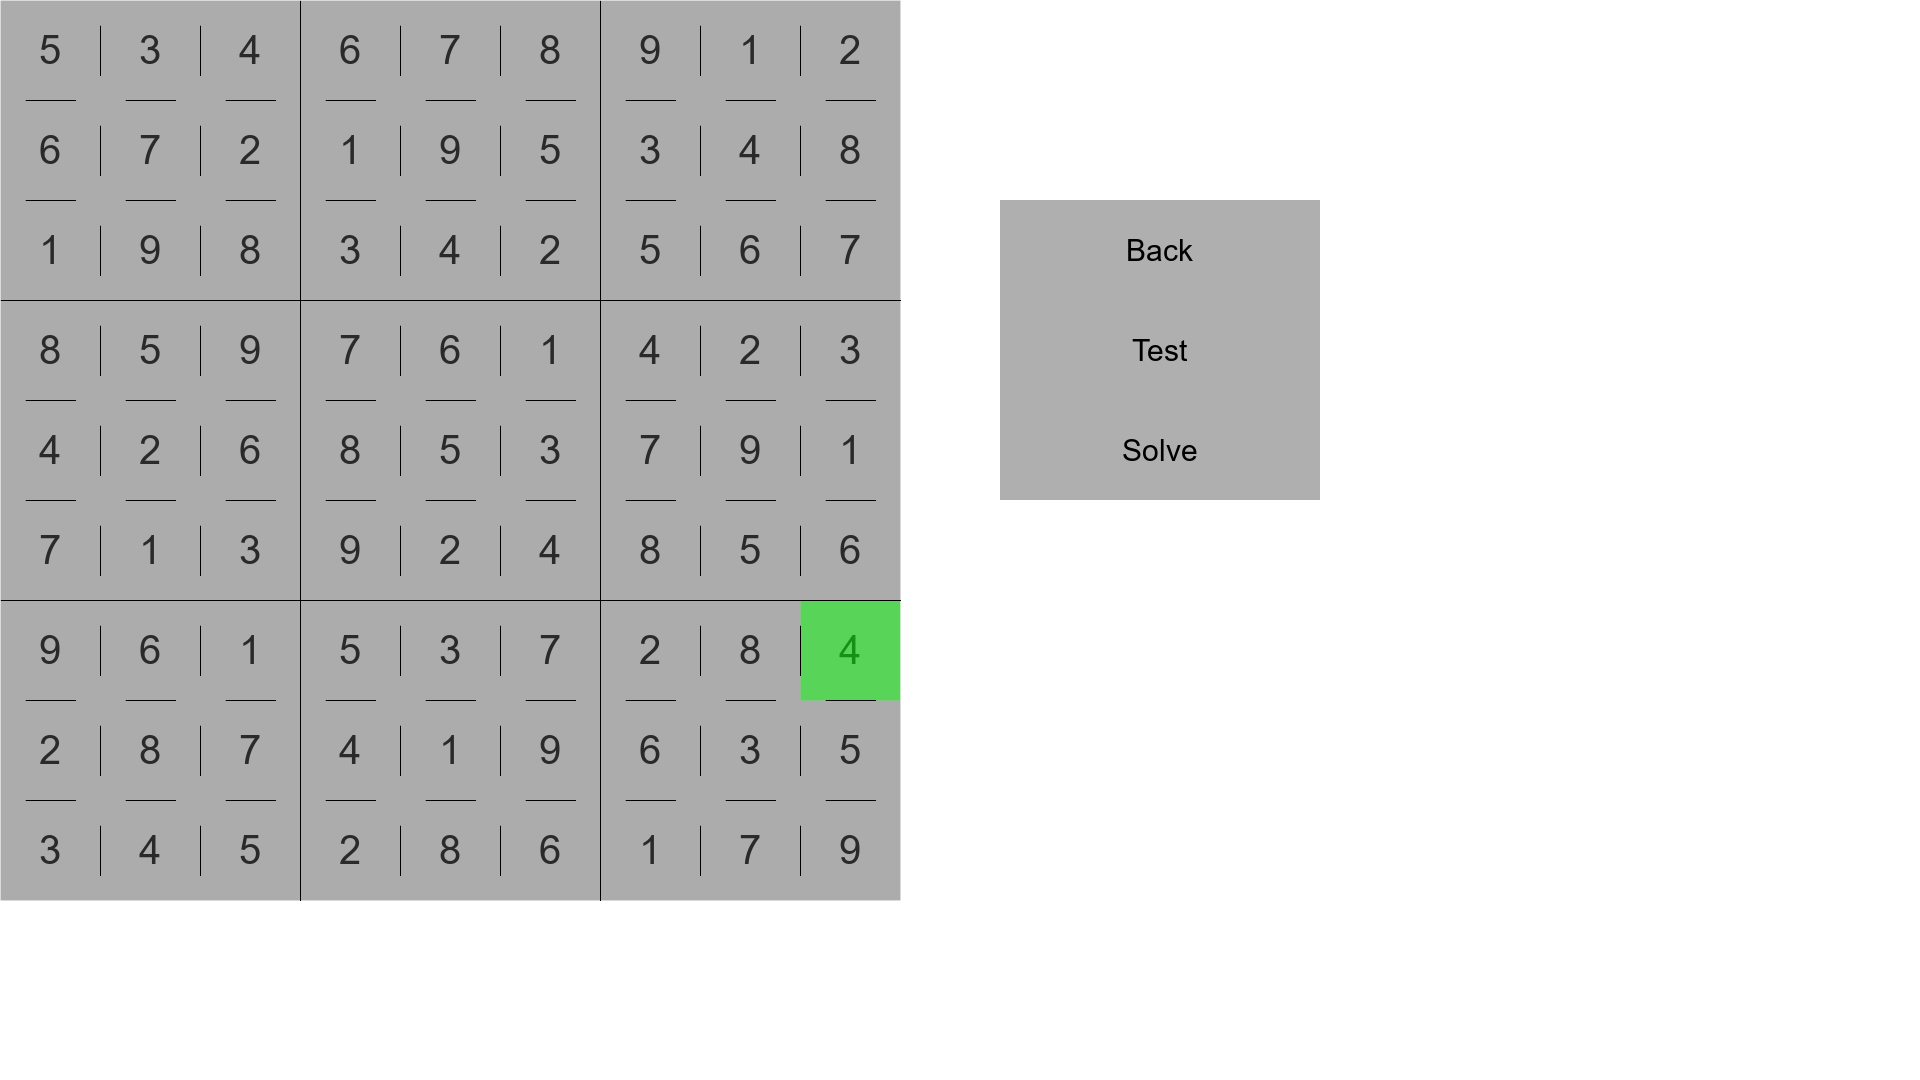
\includegraphics[width=14cm]{solver} 
	}
	\caption{\label{fig:solver} Solver.}
\end{figure}

\label{endpage}



\end{document}

%\end{article}
